\documentclass[../Main.tex]{subfiles}

\begin{document}
Amazingly, while there are infinitely many regular 2-dimensional polygons (triangles, squares, hexagons, and many more), in 3 dimensions there are only 5 \textit{platonic solids}: the most regular 3-dimensional shapes.
\begin{definition}{Platonic solid}
    A convex polyhedron $X \in R^3$ is a \underline{platonic solid} if the following are true:
    \begin{enumerate}
        \item Every face is a regular $n$-gon, and all the faces are the same
        \item The isometry group, $G = Isom(X)$, acts transitively on faces
        \item If $x \in X$ is the midpoint of a face, then $Stab_G(x) \cong D_{2n}$.
    \end{enumerate}
\end{definition}
The 5 platonic solids are, up to similarity (isometries and scaling): % TODO: draw these?
\begin{itemize}
    \item The tetrahedron: 4 triangular faces and 4 vertices
    \item The cube: 6 square faces and 8 vertices
    \item The octahedron: 8 triangular faces and 6 vertices
    \item The dodecahedron: 12 pentagonal faces and 20 vertices
    \item The icosahedron: 20 triangular faces and 12 vertices (not pictured)
\end{itemize}
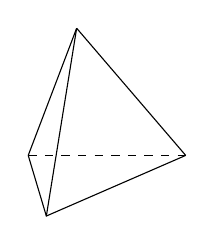
\begin{tikzpicture}[scale=2] % Tetrahedron
    \draw (0, 0, 0) -- (0.5, 0, 1) -- (1, 0, 0);
    \draw[dashed] (0, 0, 0) -- (1, 0, 0);
    \draw (0, 0, 0) -- (0.5, 1, 0.5);
    \draw (1, 0, 0) -- (0.5, 1, 0.5);
    \draw (0.5, 0, 1) -- (0.5, 1, 0.5);
\end{tikzpicture}
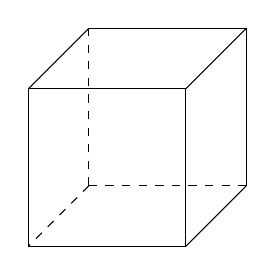
\begin{tikzpicture}[scale=2] % Cube
    \draw[dashed] (0, 0, 0) -- (1, 0, 0);
    \draw[dashed] (0, 0, 0) -- (0, 1, 0);
    \draw[dashed] (0, 0, 0) -- (0, 0, 1);
    \draw (0, 0, 1) -- (1, 0, 1) -- (1, 1, 1) -- (0, 1, 1) -- cycle;
    \draw (1, 0, 1) -- (1, 0, 0);
    \draw (1, 1, 1) -- (1, 1, 0);
    \draw (0, 1, 1) -- (0, 1, 0);
    \draw (0, 1, 0) -- (1, 1, 0) -- (1, 0, 0);
\end{tikzpicture}
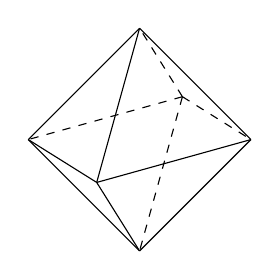
\begin{tikzpicture}[scale=2] % Octahedron
\coordinate (A) at (0, 0, 0.707);
\coordinate (B) at (0.707, 0, 0);
\coordinate (C) at (0, 0, -0.707);
\coordinate (D) at (-0.707, 0, 0);
\coordinate (E) at (0, 0.707, 0);
\coordinate (F) at (0, -0.707, 0);

\draw[dashed] (C) -- (B);
\draw[dashed] (C) -- (D);
\draw[dashed] (C) -- (E);
\draw[dashed] (C) -- (F);
\draw (A) -- (B);
\draw (A) -- (D);
\draw (A) -- (E);
\draw (A) -- (F);
\draw (B) -- (E);
\draw (B) -- (F);
\draw (D) -- (E);
\draw (D) -- (F);
\end{tikzpicture}
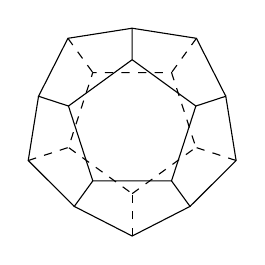
\begin{tikzpicture} % Dodecahedron
% Vertices of the dodecahedron
\coordinate (A1) at (0, 0);
\coordinate (A2) at (1, 0);
\coordinate (A3) at (1.309, 0.951);
\coordinate (A4) at (0.5, 1.539);
\coordinate (A5) at (-0.309, 0.951);

\coordinate (B1) at (-0.235, -0.324);
\coordinate (B2) at (1.235, -0.324);
\coordinate (B3) at (1.689, 1.075);
\coordinate (B4) at (0.5, 1.939);
\coordinate (B5) at (-0.689, 1.075);

\coordinate (C1) at (0.5, -0.7);
\coordinate (C2) at (1.820, 0.259);
\coordinate (C3) at (1.316, 1.811);
\coordinate (C4) at (-0.316, 1.811);
\coordinate (C5) at (-0.820, 0.259);

\coordinate (D1) at (0.5, -0.162);
\coordinate (D2) at (1.309, 0.425);
\coordinate (D3) at (1, 1.376);
\coordinate (D4) at (0, 1.376);
\coordinate (D5) at (-0.309, 0.425);

% Front pentagon
\draw (A1) -- (A2) -- (A3) -- (A4) -- (A5) -- cycle;

% Outer pentagons
\draw (A1) -- (B1) -- (C1) -- (B2) -- (A2);
\draw (B2) -- (C2) -- (B3) -- (A3);
\draw (B3) -- (C3) -- (B4) -- (A4);
\draw (B4) -- (C4) -- (B5) -- (A5);
\draw (B5) -- (C5) -- (B1);

% Back connections
\draw[dashed] (C1) -- (D1);
\draw[dashed] (C2) -- (D2);
\draw[dashed] (C3) -- (D3);
\draw[dashed] (C4) -- (D4);
\draw[dashed] (C5) -- (D5);

% Back pentagon
\draw[dashed] (D1) -- (D2) -- (D3) -- (D4) -- (D5) -- cycle;
\end{tikzpicture}\par
The icosahedron is not pictured above, since it is a very complex shape. However, we have a very interesting property that means we do not need to think about it.
\begin{definition}{Dual solids}
    Two solids $X, Y$ are \underline{dual} if $Y$ can be constructed as the convex hull of the centres of the faces of $X$.
\end{definition}
For example, an octahedron is formed by joining lines between the centres of the faces of a cube. See figure~\ref{figCubeDual}. Thus, the cube and octahedron are dual. Note that if the same process is done to the octahedron, a cube is formed.\par
We see that a necessary condition for duality is therefore that the number of faces of $X$ is the number of vertices of $Y$, and the number of vertices of $X$ is the number of faces of $Y$.
\begin{figure}[ht]
    \centering
    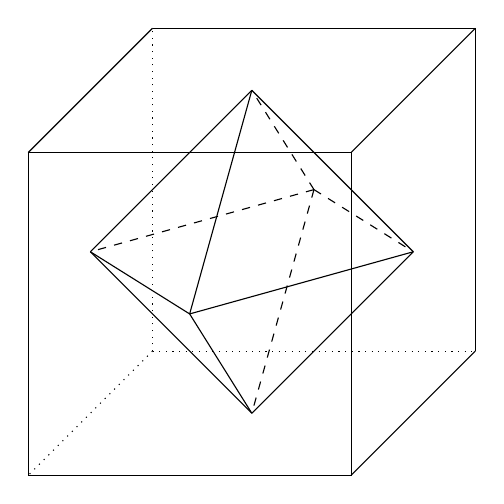
\begin{tikzpicture}[scale=4.1]
        % Draw the cube
        \draw[dotted] (0, 0, 0) -- (1, 0, 0);
        \draw[dotted] (0, 0, 0) -- (0, 1, 0);
        \draw[dotted] (0, 0, 0) -- (0, 0, 1);
        \draw (0, 0, 1) -- (1, 0, 1) -- (1, 1, 1) -- (0, 1, 1) -- cycle;
        \draw (1, 0, 1) -- (1, 0, 0);
        \draw (1, 1, 1) -- (1, 1, 0);
        \draw (0, 1, 1) -- (0, 1, 0);
        \draw (0, 1, 0) -- (1, 1, 0) -- (1, 0, 0);

        % Centres of faces. Faces named as in cubing algorithms
        \coordinate (D) at (0.5, 0, 0.5);
        \coordinate (F) at (0.5, 0.5, 1);
        \coordinate (L) at (0, 0.5, 0.5);
        \coordinate (R) at (1, 0.5, 0.5);
        \coordinate (B) at (0.5, 0.5, 0);
        \coordinate (U) at (0.5, 1, 0.5);

        % Draw the octahedron
        \draw (D) -- (F);
        \draw (D) -- (L);
        \draw (D) -- (R);
        \draw (F) -- (L);
        \draw (F) -- (R);
        \draw (U) -- (F);
        \draw (U) -- (L);
        \draw (U) -- (R);

        \draw[dashed] (B) -- (D);
        \draw[dashed] (B) -- (L);
        \draw[dashed] (B) -- (R);
        \draw[dashed] (B) -- (U);
    \end{tikzpicture}
    \caption{A cube with the octahedron drawn by connecting centres of faces.}
    \label{figCubeDual}
\end{figure}
\begin{example}
    The tetrahedron is dual to itself. Note that the number of vertices and faces is the same, so we satisfy the necessary condition.
\end{example}
We also see that the dodecahedron and icosahedron are dual.\par
Note that if $X$ and $Y$ are dual, then their isometry groups are isomorphic to each other. Therefore, we only need to think about 3 groups (tetrahedron, cube, dodecahedron), to cover all 5 solids.
\section{Symmetries of a Tetrahedron}
\begin{example}[Symmetries of a tetrahedron] % TODO: Change to lemma
    Let $G$ be the isometry group of the tetrahedron. By the definition of a platonic solid, $G$ acts transitively on faces (or midpoints thereof), and each face has stabiliser $D_6$. Therefore, by \ref{thmOrbitStab},
    \begin{equation*}
        |G| = 4 \times 6 = 24
    \end{equation*}
    Furthermore, the action on the 4 vertices defines a homomorphism:
    \begin{equation*}
        \theta : G \mapsto S_4
    \end{equation*}
    And since they are the same size, we need only prove one of surjectivity, and injectivity.\par
    \underline{Claim:} $\theta$ is injective.\par
    \underline{Proof:} We need to prove $\ker(\theta) = \{e\}$.\par
    Suppose $\theta(g) = e$, then $g$ fixes the 4 non-coplanar vertices, so $g = Id_X$ by the 4-point lemma, so $\theta$ is injective.
    Therefore, since $|G| = |S_4|, G \cong S_4$.
\end{example}
Let $G_0$ be $G \cap SO(3)$, the index-two subgroup of rotational symmetries.
\begin{lemma}[Uniqueness of $A_n$]
    If $H \leq S_n$, and $|S_n : H| = 2$\par
    Then $H = A_n$
\end{lemma}
\begin{proof}
    An index-two subgroup is always normal, so $H \normalin S_n$. Therefore, $S_n / H \cong C_2$. We therefore have a surjective homomorphism:
    \begin{equation*}
        \phi : S_n \mapsto C_2 = \{\pm 1\}
    \end{equation*}
    With $H = \ker{\phi}$. Since transpositions generate $S_2$, some transposition $\tau_0$ has $\phi(\tau_0) = -1$. But all transpositions are conjugate, so $\tau = \sigma \tau_0 \sigma^{-1}$ for any transposition $\tau$. Now:
    \begin{align*}
        \phi(\tau) &= \phi(\sigma \tau_0 \sigma^{-1}) \\
        &= \phi(\sigma) \phi(\tau_0) \phi(\sigma^{-1}) \\
        &= \phi(\sigma) \phi(\sigma^{-1}) \phi(\tau_0) \text{ since } C_2 \text{ is abelian} \\
        &= \phi(\tau_0) = -1
    \end{align*}
    Therefore $\phi = sign$, and so $H = A_n$.
\end{proof}
So we know that our group $G_0 \cong A_4$.
\section{Symmetries of a Cube}
\begin{lemma}
    The group of isometries of a cube, $G = Isom(X)$, is isomorphic to $S_4 \times C_2$.
\end{lemma}
\begin{proof}
    Using Theorem~\ref{thmOrbitStab},
    \begin{equation*}
        |G| = 6 \times 8 = 48
    \end{equation*}
    And the index-two rotational subgroup $G_0$ has order $24$.\par
    From Ex2Q7, $G$ acts on the set of 4 long diagonals in $G$, and we thus obtain a homomorphism
    \begin{equation*}
        \theta : G_0 \mapsto S_4
    \end{equation*}
    We then show that this homomorphism is surjective. Since transpositions generate $S_4$, it suffices to show that all transpositions are in the image of $\theta$. Indeed, rotation about the axis through the midpoints of two opposite edges maps to a transposition in $S_4$. There are 6 such rotations, and there are transpositions in $S_4$, so we have surjectivity.\par
    Now $\theta$ is a surjective homomorphism and the groups are the same size, so $\theta$ is an isomorphism, and $G_0 \cong S_4$.\par
    We then consider the isomorphism $-Id_X$, that sends all vectors (considering the centre of the cube as the origin) to their negatives. Now $-Id_X \notin S_4$ and $-Id_X$ commutes with everything, so we can apply the direct product theorem: $G \cong S_4 \times C_2$.
\end{proof}
\section{Symmetries of a Dodecahedron*}
*Note that the content of this section is \textbf{non-examinable}.
\begin{lemma}
    Let $X \in A_5$ be the set of 3-cycles. Then
    \begin{equation*}
        \langle X \rangle = A_5
    \end{equation*}
    \label{lem3CyclesGenerateA5}
\end{lemma}
\begin{proof}
    Recall that $X$ is a conjugacy class in $A_5$. By Ex4Q3, $\langle X \rangle \normalin A_5$. But from Theorem~\ref{thmA5Simple}, $\langle X \rangle$ must be the whole of $A_5$.
\end{proof}
\begin{figure}[hb]
    \centering
    \includegraphics[scale=0.4]{{Cubes inside dodecahedron}}
    \caption{Edges of cubes drawn onto a dodecahedron}
    \label{figCubesOnDodec}
\end{figure}
\begin{lemma}[Symmetries of a dodecahedron]
    The symmetry group of a dodecahedron, $G$, is isomorphic to $A_5 \times C_2$.
\end{lemma}
\begin{proof}
    Let $G_0$ be the index-$2$ rotational subgroup in $G$.\par
    Since a face has orbit of size $12$ (from the $12$ faces), and stabiliser isomorphic to $D_{10}$ (the faces are pentagons), from theorem~\ref{thmOrbitStab} we get that $|G| = 12 \times 10 = 120$, and so $|G_0| = 60$.\par
    By drawing diagonals on faces, we may inscribe 5 cubes into the dodecahedron. See figure~\ref{figCubesOnDodec}.\par
    This action on the 5 cubes leads to a homomorphism:
    \begin{equation*}
        \theta : G_0 \mapsto S_5
    \end{equation*}
    In the action, every rotation about an axis through an opposite pair of vertices is a 3-cycle with respect to the cubes. Each such axis is the axis for 2 rotations of angles $\pm\frac{\pi}{3}$. Each such rotation maps to a 3-cycle in $S_5$ under $\theta$, and there are 20 of them. That is, $\begin{pmatrix}5 \\ 3\end{pmatrix} \times 2$, which is all the 3-cycles in $S_5$. Then by lemma~\ref{lem3CyclesGenerateA5}, we must have that $A_5 \leq \im{\theta}$. Therefore, since $G_0$ and $A_5$ have the same size, $G_0 \cong A_5$.\par
    Now, we use the same argument as for the cube to show $G \cong A_5 \times C_2$.
\end{proof}
\end{document}